\documentclass[12pt,onecolumn,letterpaper,draftclsnofoot]{article}
% \documentstyle[12pt]{article}

% \usepackage{fullpage}

\usepackage{cvpr}
\usepackage{times}
\usepackage{epsfig}
\usepackage{graphicx}
\usepackage{amsmath}
\usepackage{amssymb}
\usepackage{booktabs}
\usepackage{multirow}
\usepackage{subcaption}
\usepackage{scrextend}
\usepackage{bm}

% Include other packages here, before hyperref.

% If you comment hyperref and then uncomment it, you should delete
% egpaper.aux before re-running latex.  (Or just hit 'q' on the first latex
% run, let it finish, and you should be clear).
\usepackage[breaklinks=true,bookmarks=false]{hyperref}

\DeclareGraphicsExtensions{.pdf,.jpg,.png,.jpeg}
\graphicspath{{images/}, {figs/}}
\newcommand{\todo}[1]{\textcolor{red}{{\em [#1]}} }
\newcommand{\specialcell}[2][c]{%
    \begin{tabular}[#1]{@{}c@{}}#2\end{tabular}}
\newcommand{\secref}[1]{Section~\ref{sec:#1}}
\newcommand{\figref}[1]{Figure~\ref{fig:#1}}
\newcommand{\tabref}[1]{Table~\ref{tab:#1}}
\newcommand{\equref}[1]{Equation~\ref{equ:#1}}
\newcommand{\matr}[1]{\mathbf{#1}}
\newcommand{\bfit}[1]{\boldsymbol{#1}}
\newcommand{\bs}[1]{\boldsymbol{#1}}

\DeclareMathOperator*{\argmax}{arg\,max}
\DeclareMathOperator*{\argmin}{arg\,min}

\cvprfinalcopy % *** Uncomment this line for the final submission

\def\cvprPaperID{****} % *** Enter the CVPR Paper ID here
\def\httilde{\mbox{\tt\raisebox{-.5ex}{\symbol{126}}}}

% Pages are numbered in submission mode, and unnumbered in camera-ready
%\ifcvprfinal\pagestyle{empty}\fi
\begin{document}

%%%%%%%%% TITLE
\title{Survey on Recent Image and Video Captioning}

\author{Weilian Song\\
University of Kentucky\\
{\tt\small weilian.song@uky.edu}
% For a paper whose authors are all at the same institution,
% omit the following lines up until the closing ``}''.
% Additional authors and addresses can be added with ``\and'',
% just like the second author.
% To save space, use either the email address or home page, not both
}

\maketitle
%\thispagestyle{empty}

%%%%%%%%% BODY TEXT
\section{Introduction}

Automatic image and video captioning is a relatively new field in the field of
machine learning, in which a program learns to automatically assign a
sentenced-description of an image, or in the case of a video, for every frame.
Desite being new, this technology has improved itself over the past three
years and is widely used in today's world, from automatically generating video
captions for Youtube videos to clustering images/videos based on their
captions.

In this survey, we will introduce basic concepts of a nerual image/video
caption generator, which include topics like Recurrent Neural Networks (RNN),
Long-Short-Term-Memory (LSTM), and a baseline model in which researchers
expand upon. We will also explain various evaluation methods that researchers
use to compare their models with others.

Next we explore two expansions made to the naive method, one through the use
of an attention mechanism, and the other through the process of dense
labelling. Four recent papers from CVPR and ICCV are chosen as
representatives, two for each expansions. Each pair utilizes the same general
concepts, but are different in their approach.

%-------------------------------------------------------------------------
\section{Background Information}

\subsection{Multilayer Perceptrons}
\todo{Cite the data science blog post on MLP}

Multilayer perceptron, or MLP for short, is the building block for a lot of
modern neural networks. MLP consists of many layers of neurons, with each
neuron in a layer connected to every other node in its neighboring layers,
associating each edge with a weight, as shown in \figref{mlp}. In a simple,
non-recurrent MLP, the connected nodes together make an acyclic graph with the
left side as inputs and right side as outputs. 
 
\begin{figure}
  \centering
  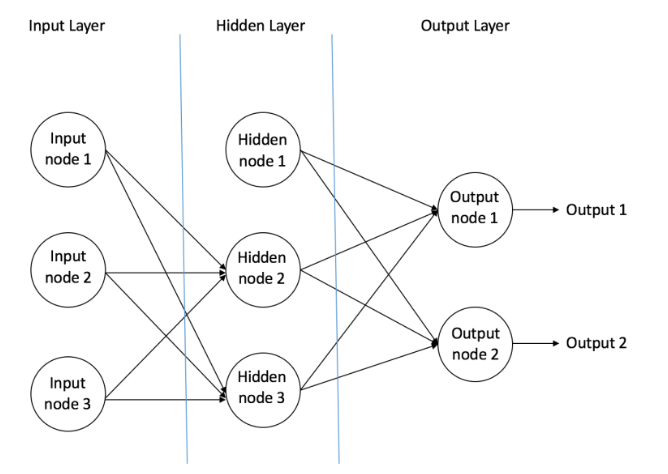
\includegraphics[width=0.6\linewidth]{networks/mlp}
  \caption{Simple MLP with one hidden layer, borrowed from \cite{datasciencemlp}}
  \label{fig:mlp}
\end{figure}
 
When we provide an input, each neuron computes a weighted sum of all of its
inputs, and combined with a bias term, the output passes through an activation
function, which introduces non-linearity, and becomes the neuron's output.
Neurons are updated from left to right, and the outputs of the rightmost
neurons becomes the network output.

Learnable parameters include the weights for each edge between neurons and the
bias term for each hidden layer. In \figref{mlp}, hidden node 1 is the bias
term for the hidden layer.

\subsection{Recurrent Neural Networks}

Recurrent Neural Networks, or RNN for short, are a class of neural networks
that make use of previous network outputs for the next immediate prediction.
They are able to maintain long-term dependencies between predictions, which is
useful in fields like nautral language processing, where prediction at the
current time step is recursively dependent upon previous predictions.

Borrowing definition from \cite{deeplearning4jrnn}, assuming a recurrent
neural network of only one layer with input $\bm{x}$, layer weights $\bm{W}$,
and output $\bm{y}_{t-1}$ at time step $t-1$, we can define our network output
$\bs{y}$ at time step $t$ as:
%
\begin{equation}
  \bs{y}_t = \phi (\bm{W} \matr{x_t} + \bm{U} \bs{y}_{t-1})
\end{equation}
%
where $\phi$ is an activation function that squashes the values in the
parentheses into a specified range, and $\bm{U}$ is the transition matrix
between hidden states and the concept of hidden-states to hidden-states is
similar to a Markov chain.

As we can see, our network output at timestep $t$ is depend upon the regular
feedforward section of the network $\bm{W} \bm{x_{t}}$ and some information
about its past outputs, which is obtained with $\bm{U} \bm{y}_{t-1}$. $\bm{U}$
is a learnable matrix that learns what and how much previous outputs should the
network apply to the current prediction.

Extending this simple example to a network with multiple and different types
of layers, our layer's output will not be $\bs{y}$ anymore, instead it
will become hidden, not directly observable, which we denote as
$\bs{h}$. The rest of the equation remains the same, and multiple
recurrent neural layers can be stacked for more complex models.

%When backpropagating the error through the network and updating the learnable
%parameters of the recurrent layers, the gradient calculation is comparable to
%a feed-forward network, except the fact that the layer's output is the result
%of a series of chain rules. Calculus is again used but no special exceptions
%are made for recurrent layers.

One major issue with vanilla RNN is that during optimization, any small change
to the weights can become very large after many updates, similar to how
multiplying a number by $0.1$ many times will cause the number to approach 0
very fast. This is known as the vanishing or exploding gradient problem, and
as a solution to this issue, LSTM units are born.

\subsection{Long Short-Term Memory Units}
Long Short-Term Memory units, or LSTM for short, are a special kind of RNN.
It mainly resolves the issue of long-term dependencies between predictions
using a series of gates to remove and insert information between time steps.
 
\begin{figure}
  \centering
  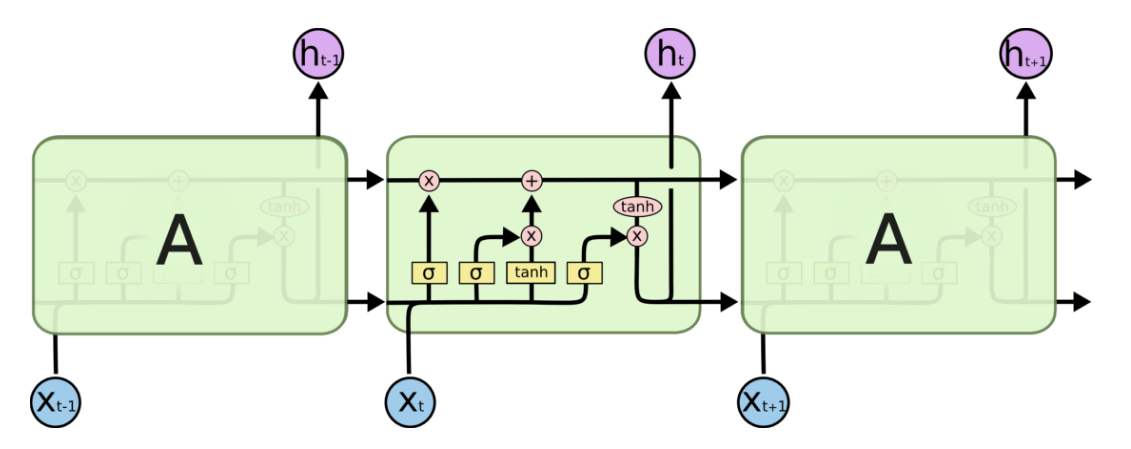
\includegraphics[width=0.8\linewidth]{networks/lstm}
  \caption{Inside of a LSTM unit, borrowed from \cite{colahlstm}}
  \label{fig:lstm}
\end{figure}
 
Borrowing \figref{lstm} from \cite{colahlstm}, we see the inner components of
an LSTM unit. There is the addition of a cell state variable $C_t$, which is
the line running across the top of the LSTM unit, and three learnable $\sigma$
(sigmoid) gates and one $\tanh$ gate that control $C_t$ from LSTM units to
LSTM units, depicted in yellow rectangles. The left most sigmoid gate controls
what information to forget from $C_t$ based on $h_{t-1}$, the middle sigmoid
and $\tanh$ gate determines what new information to add to $C_t$ based on
$h_{t-1}$, and the right most sigmoid gate generates the output $h_t$, which
is a combimation of $C_t$ and $h_{t-1}$. $C_t$ and $h_t$ are then passed to
the cell at timestep $t+1$, and the process repeats.

\subsection{Basic Image/Video Captioning Model}

\todo{Provide a basic image/video captioning model to reference back to}

\subsection{Evaluation Methods}

For evaluation of image/video captioning systems, there are three popular
metrics: BLEU, METEOR and CIDEr. \todo{cite the three metrics}

\paragraph{BLEU}
BLEU aims at computing the similarity percentage between the candidate
(predicted) sentences and all reference sentences by finding the maximum
overlap between any candidate-reference pair, looking at $n$-grams up to a
specific $n$. A $n$-gram is any phrase that is $n$ words long, and the larger
the $n$, the higher level of coherence required between $n$ words. BLEU uses
the precision scores of $n$-grams combined with a brevity penalty, which
penalizes if the candidate is shorter than the reference. This metric
does not care about the ordering of $n$-grams, so even if the score for a
sentence is high, it still might not sound natural to a human.

\paragraph{METEOR}
METEOR addresses several issues that BLEU has, mainly the lack of recall in
the calculation of the score and forced matching of only exact words instead
of synonyms also. Instead of comparing $n$-grams, each word in the candidate
sentence is matched with at most one word in the reference sentence, with
exact words matched first, followed by words with similar parts (stem) and
meanings (synonyms). The METEOR score is then calculated based on precision
and recall scores of single-word matches, weighted by a fragmentation fraction
that proportionally penalizes the score based on incorrect ordering of the
words.

\paragraph{CIDEr}
CIDEr is similar to BLEU in that it also compares $n$-grams between
candidate-reference pairs, except that it computes the cosine similarity
instead of just precision, which accounts for both precision and recall. In
addition, CIDEr enforces that $n$-grams not present in reference should not
appear in candidate, and $n$-grams that are common among references should
have less influence, as they most likely don't provide any useful information
for scoring.

\section{Attention Mechanism}

The use of an attention mechanism has become popular in image and video
captioning. Basic concept is that at each training iteration, the network
learns to focus on specific image regions to extract more useful information
than the global image representation. Below are two attention mechanisms
recently introduced, and we will be taking a look at each one and compare
their results on a common dataset.

\subsection{Knowing When To Look}
Lu et.\ al.\cite{attentionwhen} proposes a novel mechanism that learns not only
\textit{what} to look but \textit{when} as well. If the model chooses to not
attend to the image, it uses the language model stored in the RNN instead.
The proposed network extends the CNN-RNN model, using ResNet \cite{resnet} as
their CNN network, LSTM as their RNN of choice and inserting their attention
mechanism in between the CNN and RNN.

For the network to learn when to focus on specific regions and when to refer
to the language model, the authors propose a new context vector $\hat{c}_t$ to
be used for the RNN, calculated as follows, borrowing equation from
\cite{attentionwhen}:
%
\begin{equation}
  \hat{\bm{c}}_t = \beta_t \bm{s}_t + (1 - \beta_t) \bm{c}_t
\end{equation}
%
with $\bm{s}_t$ being the visual sentinel (language model), $\bm{c}_t$ being
the attention-focused image feature, and $0 \le \beta_t \le 1$ as the gate
parameter that controls the mixture of the two features. When $\beta_t=1$, the
network would have essentially turned the attention mechanism off and use only
the visual sentinel features, and vice versa.

The visual sentinel $\bm{s}_t$ is calculated as a function of the LSTM input
$\bm{x}_t$, hidden state $\bm{h}_t$, and cell state $\bm{m}_t$. The
attention-focused image feature $\bm{c}_t$ is calculated as a weighted sum of
image spatial features $\bm{V}$, with the weights learnable and dependent on
$\bm{V}$ and $\bm{h}_t$. $\bm{V}$ is obtained from the last layer of ResNet
\cite{resnet} followed by a single layer perceptron.

% In their proposed model, an encoder takes in an input image and outputs a
% context vector $\bs{c}_t$, which is the output of a trained image
% classification network and provides visual features for caption generating.
% $\bs{c}_t$ is then fed into a LSTM unit, followed by a novel attention
% mechanism and a MLP for the final prediction.  \todo{maybe a diagram here?
% Also this is wrong}
% 
% The novel attention mechanism that Lu et. al. introduces is a variation of
% soft attention model from ??? \todo{cite}. To compute the context vector
% $\bs{c}_t$, they define it as:
% %
% \begin{equation}
%   \bs{c}_t = g(\matr{V}, \bs{h}_t)
% \end{equation}
% %
% where $\matr{V} = [\mathbf{v}_1,\dots,\mathbf{v}_k], \mathbf{v}_i \in R^d$
% \todo{fix real numbers} is the image feature divided into $k$ areas and each
% area having $d$ dimensions. $g$ is the attention mechanism the author
% proposes, which is a single layer neural network computing the attention
% distrubtion of the $k$ areas of the image:
% %
% \begin{align}
%   \matr{z}_t &= \matr{w}_h^T \tanh(\matr{W}_v \matr{V} + \matr{W}_g \matr{h}_t) \\
%   \alpha_t   &= \operatorname{softmax}(\matr{z}_t)
% \end{align}
% %
% where \todo{a lot of explaining here...}, and $\alpha \in R^k$ is the
% attention weight over $k$ areas of the image feature $\matr{V}$. With
% $\alpha_t$, we can compute the context vector as:
% %
% \begin{equation}
%   \bs{c}_t = \sum_{i=1}^k \alpha_{ti} \bs{v}_{ti}
% \end{equation}
% %
% and finally we have a MLP layer $f$ that computes the probability distribution
% over words:
% %
% \begin{equation}
%   \log p(y_t | y_1,\dots,y_{t-1},I) = f(\bs{h}_t, \bs{c}_t)
% \end{equation}
% %
% Overview of the attention network is shown in ???, which is borrowed from the
% original text.
% 
% Authors also propose a method for allowing the network to choose features
% produced by the attention system or another set of features
% $\bs{s}_t$, the ``visual sentinel''. It is calculated as follows:
% %
% \begin{align}
%   \bs{g}_t &= \sigma (\bfit{W}_x \bs{x}_t + \bfit{W}_h \bs{h}_{t-1} \\
%   \bs{s}_t &= \bs{g}_t \odot \tanh (\bs{m}_t)
% \end{align}
% %
% where $\bfit{W}_x$ and $\bfit{W}_h$ are again weights to be learned and
% $\bs{m}_t$ is the LSTM cell state. Combining with the attention
% mechanism output $\bs{c}_t$, we have:
% %
% \begin{equation}
%   \hat{\bs{c}}_t = \beta_t \bs{s}_t + (1 - \beta_t) \bs{c}_t
% \end{equation}
% %
% where $\beta_t$ is our sentinel gate and is between 0 and 1 to control how
% much information to use from each. When $\beta_t=1$, we essentially turn
% off the attention mechanism and only use the visual sentinel feature, vice
% versa. \todo{maybe explain that it's inspired by residual nets}

\subsection{Areas of Attention for Image Captioning}

Pedersoli et.\ al.\cite{attentionwhere} proposes a novel attention mechanism
that associates areas of interest when generating captions. When predicting
the word at each time step, the network learns the relationship between the
predicted words, areas of interest, and the hidden state of the RNN through a
triangular relationship, as shown in \figref{triangle}.
%
\begin{figure}
  \centering
  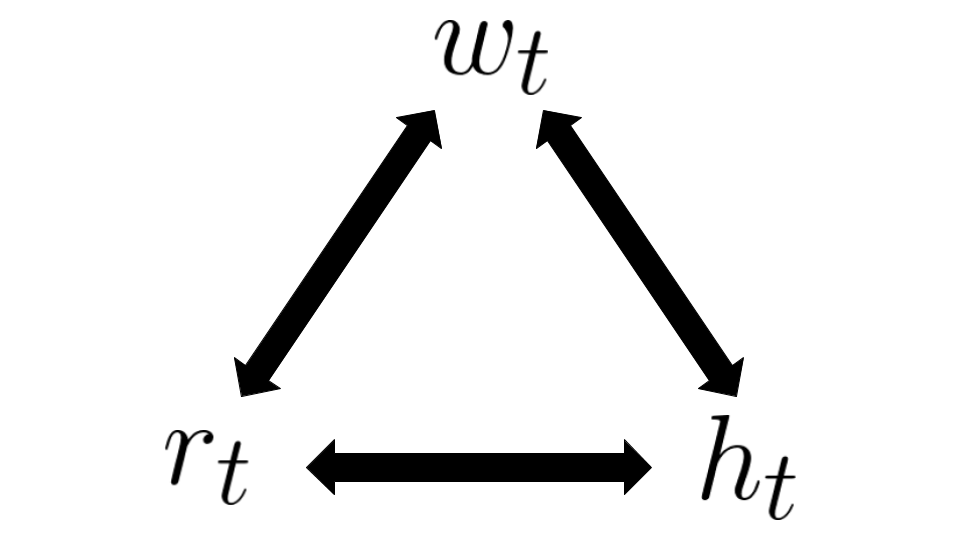
\includegraphics[width=0.4\linewidth]{traingle}
  \caption{Triangular relationship between predicted words (top), image
  regions (bottom left), and hidden state of GRU (bottom right)}
  \label{fig:triangle}
\end{figure}
%
For comparison, a vanilla RNN model for image captioning only finds the
relationship between words and the hidden state of the RNN.
  
The proposed network is a modified CNN-RNN network, using VGG16 as its CNN and
gated recurrent units (GRU), which are similar to LSTM units. There are three
main learnable parameters within the network, $\theta_{wh}$, $\theta_{wr}$,
and $\theta_{rh}$.  Simplifying the equations shown in \cite{attentionwhere},
we can compute the joint distribution over words and image regions as follows:
%
\begin{equation}
  \begin{aligned}
    p(w_t, r_t|h_t) &\propto \exp s(w_t, r_t, h_t) \\
    s(w_t, r_t, h_t) &= f(w_t, h_t, \theta_{wh}, W) \\
                     &+ f(w_t, r_t, \theta_{wr}, W, R) \\
                     &+ f(r_t, h_t, \theta_{rh}, R) \\
                     &+ bias
  \end{aligned}
\end{equation}
%
where $r_t$ encodes the image regions the network attends to at time $t$ and
$W,R$ are word and region representations. Function $s(w_t, r_t, h_t)$ is the
summation of three terms, computing the relationship between words and hidden
state, words and image regions, and image regions and hidden state,
respectively. The last term is a linear bias that is learnable by the network.

Given the hidden cell state, the predicted word at time $t$ is computed
through the word distribution $p(w_t|h_t) = \sum_{r_t} p(w_t,r_t|h_t)$. The
authors also utilize the predicted probability distribution over regions
$p(r_t|h_t)$ to provide a feedback signal to the RNN for the next word
prediction, which they denote as $v$. It is a form of weakly-supervised
learning, as in the network is using its own predictions as labels to train.

In regards to the image regions $r$, authors have experimented with three
different types: activation grid (fixed size square bounding boxes), object
proposals (bounding boxes around objects), and spatial transformers
(transformed activation grids). The image regions are obtained from outputs of
the last few layers of VGG16 during training.

\subsection{Attention Mechanisms Evaluation}
\tabref{attention} shows the evaluation of the two attention mechanisms using
COCO \cite{coco}, the largest image captioning dataset from Microsoft. Lu et.\
al.'s knowing \textit{when} to look attention mechanism outperforms Pedersoli
et.\ al.'s knowing \textit{where} to look attention mechanism. It is worth
noting that Pedersoli et.\ al.\ does not claim that they are the
state-of-the-art, but the new mechanism that the authors have proposed can be
integrated into a lot of existing state-of-the-art networks. Lu et.\ al.\ also
analyzed their network's ability to learn \textit{where} to attend, however the
evaluation is minimal compared to Pedersoli et.\ al.'s method, so it would be
very interesting to combine the two methods to see how it performs.
%
\begin{table}[]
\centering
\caption{Various evaluation scores for the two attention mechanisms}
\label{tab:attention}
\begin{tabular}{llll}
	\toprule
	Method         & BLEU-4         & METEOR         & CIDEr          \\
	\hline
	Attention Area & 0.307          & 0.245          & 0.938          \\
	Attention When & \textbf{0.332} & \textbf{0.266} & \textbf{1.085} \\
	\bottomrule
\end{tabular}
\end{table}
%
\section{Dense Labeling}

While one caption for one image/video is a remarkable step for neural networks
in imagery understanding, it forces the network output to be of global
context. For example, a picture of a park with lots of people in it would most
likely have a caption of ``People of all ages are enjoying themselves in a
park.'' While it summarizes the image very well, it is limited to only
summaries and no specific information like ``A group of teenagers are playing
soccer'' or ``The weather is very nice today''.

This is where dense labeling comes in, where for a given image and bounding
boxes, the network learns to caption the image content in each bounding box.
In the case of a video, the bounding box can move with an object throughout
the frames, and the network outputs several captions for one video.

First introduced by ??? \todo{find first}, dense labeling technique has been
improved over the years. Below are two CVPR 2017 papers that has contributed
new knowledge, proposing novel techniques that solves various challenges
associated with this field..

\section{Dense Captioning with Joint Inference and Visual Context}
Yang et.\ al.\cite{denseyang} proposes a dense image captioning network, which
jointly learns to classify bounding boxes and captions of regions of interest.
The proposed architecture consists of two connected networks. First is a
region detection network, and following is a localization and captioning
network.

\paragraph{Region Detection Network}
The purpose of the region detection network (RDN) is to identify areas of high
interest for the network to generate captions. The authors use Faster R-CNN
network \cite{renNIPS15fasterrcnn} for the task. Faster R-CNN is an object
detection network that uses a Region Proposal Network (RPN) to first generate
region proposals (similar to an attention mechanism) and then detect objects
within each region. In the case of the RDN, an image is first passed through a
CNN network to generate image features. Then the features are passed through
the RPN to obtain region proposals. The convolved image features are passed
through a series of pooling layers to reduce dimensiality and finally for each
region proposals, region features are extracted from the pooled features and
serve as inputs to the localization and captioning network.

\begin{figure}
  \centering
  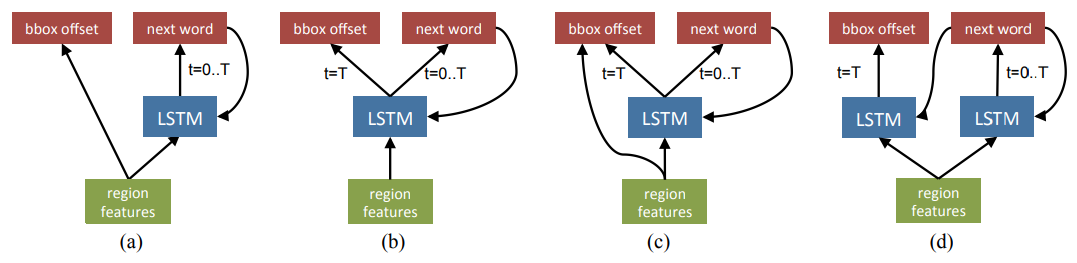
\includegraphics[width=\linewidth]{networks/densejoint}
  \caption{Different model designs for the localization and captioning
  network, borrowed from \cite{renNIPS15fasterrcnn}}
  \label{fig:densejoint}
\end{figure}

\paragraph{Localization and Captioning Network}
Using the region features as input, the network learns to predict the caption
and the bounding box offset for each region. Figure \figref{densejoint} shows
four different variations of the network, all of which uses LSTM for
generating word at each time step. The left most network is the baseline,
where the bounding box offset is not dependent upon the recurrent information
from predicting words. The second, third and fourth network are what the
authors refer as Shared-LSTM (S-LSTM), Shared-Concatenated-LSTM (SC-LSTM), and
Twin-LSTM (T-LSTM). It is important to note that the bounding box offset is
not predicted until after predicting the last word of the caption, so it can
utilize the entire chain of recurrent information for prediction.

The authors also experimented with a global context fusion technique, where
the global image feature from the CNN is passed through another set of pooling
layers to obtain the context feature and concatenated with each region feature
for caption generation. There can be early and late fusion, as in the two
features can be concatenated before or during LSTM predictions. Evaluations
are performed on the two methods as well.

\section{Weakly Supervised Dense Video Captioning}
Shen et.\ al.\cite{denseshen} approach a slightly different problem of
generating captions for videos instead of images. Their model is able to
generate multiple captions given a single video, and while it has been done
before, the main novelty is that the network is not learning from training
data that maps specific video frame regions to captions. Instead the network
extracts rough region candidates and 

\section{Conclusion}

Conclusion

{\small
\bibliographystyle{ieee}
\bibliography{biblio}
}

\end{document}
